% !TEX options=--shell-escape
% Thesis template by Julian Lueken

% Optimized for literature management with JabRef + BibLaTeX

% Change user settings:
%	"keep_focus": true, --> false, to remove the annoying pop ups
%	"use_biblatex": false,
%	"builder": "traditional" --> "basic", to use biber on every compilation

\documentclass[a4paper, 11pt]{report}

% Packages
%% Input encoding
%%\usepackage[utf8]{inputenc}
\usepackage[T1]{fontenc}
\usepackage{lmodern}

%% Languages and symbols
\usepackage[main=english]{babel}
\usepackage{extarrows}
\usepackage{marvosym}

%% AMS packages
\usepackage{amssymb}
\usepackage{amsmath}
\usepackage{amsthm}

%% Citations and references
\usepackage[style=alphabetic, backend=biber]{biblatex} 
\usepackage[hidelinks]{hyperref}
\usepackage{csquotes}
\usepackage{nameref}
\usepackage{cleveref}
\usepackage{listings}

%% Page geometry
\usepackage[onehalfspacing]{setspace}
\usepackage[top=30mm, left=25mm, right=25mm, bottom=20mm]{geometry}
\usepackage{titlesec}

%% Figures and graphics
\usepackage{graphicx}
\usepackage{xcolor}
\usepackage{colortbl}
\usepackage{subcaption}
\usepackage{tikz}
\usepackage{float}
\usepackage{svg}

%% Pseudo-code
\usepackage{algorithm}
\usepackage[noend]{algpseudocode}

%% Testing
\usepackage{lipsum}

%% Package settings
%%% BibLaTeX resource (JabRef output file)
\addbibresource{../bibtex/bibliography.bib}

%%% Hyperref options
\hypersetup{hypertexnames=false}

%%% Listings options (for writing code in LaTeX)
\lstset{numbers=left, numberstyle=\tiny, numbersep=5pt}
\lstset{language=Python}

%%% AMS environment definitions
\theoremstyle{definition}
\newtheorem{definition}{Definition}[section]
\newtheorem{example}[definition]{Example}
\newtheorem{theorem}[definition]{Theorem}
\newtheorem{corollary}[definition]{Corollary}
\newtheorem*{remark}{Remark}
\newenvironment{myAbstract}{\section*{Abstract}}{}

%%% Special formatting
\renewcommand{\emph}[1]{\textit{#1}}
\newcommand{\mytitle}[1]{\LARGE{#1}\normalsize\\[0.3em]}
\newcommand{\titlespace}{\vspace{2em}}
\newcommand{\smallspace}{\vspace{1em}}
\newcommand{\hugespace}{\vspace{17em}}
\newcommand{\logoheight}{4em}

%% Special formatting for pesudocode
\algblock{Input}{EndInput}
\algnotext{EndInput}
\algblock{Output}{EndOutput}
\algnotext{EndOutput}
\newcommand{\Desc}[2]{\State \makebox[12em][l]{#1}#2}


\begin{document}

% Chapter format
\titleformat{\chapter}[hang]{\normalfont\huge\bfseries}{\thechapter}{0.75em}{\huge\bfseries}
\titlespacing*{\chapter}{0em}{0em}{1em}

% Title page
\pagenumbering{gobble}
\newgeometry{top=35mm, left=20mm, right=20mm, bottom=10mm}
\begin{titlepage}
	\begin{center}
		\begin{minipage}{.49\textwidth}
			\flushleft
			\includegraphics[height=\logoheight]{../assets/formal/logo_gau.png}
		\end{minipage}
		\begin{minipage}{.49\textwidth}
			\flushright
			\includegraphics[height=\logoheight]{../assets/formal/logo_dlr.png}	
		\end{minipage}
		\begin{minipage}{.49\textwidth}
			\begin{center}
				\vspace{2cm}
				Master's thesis in\\
				Applied Computer Science\\
				\titlespace
				\mytitle{CoolingGen}
				A parametric 3D-modeling software for turbine blade cooling geometries using NURBS\\
				\titlespace
				\today\\
				\hugespace
				Institute for Numerical and Applied Mathematics at the Georg-August-University Göttingen\\
				\titlespace
				Institute for Propulsion Technology at the German Aerospace Center in Göttingen\\
				\titlespace
				Bachelor's and master's theses at the Center for Computational Sciences at the Georg-August-University Göttingen\\
				\titlespace
				Julian Lüken\\
				\texttt{julian.lueken@dlr.de}\\
			\end{center}
		\end{minipage}
	\end{center}
\end{titlepage}
\pagebreak

% Address page
\pagestyle{empty}
\restoregeometry
\newgeometry{top=210mm, left=45mm, right=45mm}
\noindent
\begin{tabular}{l}
Georg-August-University Göttingen\\
Institute of Computer Science\\
\end{tabular}\\[1em]
\begin{tabular}{ll}
	\Telefon 	&+49 (551) 39-172000\\
	\FAX 		&+49 (551) 39-14403\\
	\Letter 	&\texttt{office@cs.uni-goettingen.de}\\
\end{tabular}\\[1em]
\begin{tabular}{l}
\texttt{www.informatik.uni-goettingen.de}\\
\end{tabular}\\[1em]
\pagebreak

% Done-it-myself page
\noindent I hereby declare that this thesis has been written by myself and no other resources than those mentioned have been used.\\[0.7em]
\phantom{H}\includegraphics[height=3em]{../assets/formal/sign.png}\\[0.5em]
Göttingen, \today \hspace{2em}
\pagebreak

% Abstract and Zusammenfassung
\restoregeometry
\begin{abstract}
	\thispagestyle{plain}
	\pagenumbering{roman}
	\setcounter{page}{3}
	\lipsum[1-3]
\end{abstract}
\renewcommand{\abstractname}{Zusammenfassung}
\begin{abstract}
	\thispagestyle{plain}
	\pagenumbering{roman}
	\setcounter{page}{4}
	\lipsum[4-6]
\end{abstract}
\pagebreak

% Table of contents
\setcounter{page}{5}
\restoregeometry
\tableofcontents
\pagebreak

% Actual document starts here
\restoregeometry
\pagenumbering{arabic}
\setcounter{page}{1}
\pagestyle{plain}

\chapter{Introduction}
\section{Motivation}
\section{State of the Art}
\section{Problem Statement}

\chapter{Methods}
\section{Bézier Curves}
Bézier curves are named after the french engineer Pierre Bézier, who famously utilized them in the 1960s to design car bodies for the automobile manufacturer Renault \cite{Bezier1968}. Today, they are used in a wide variety of vector graphics applications (i.e. in font representation on computers). At first glance, the definition of the Bézier curve might seem cumbersome, but given the mathematical foundation and a few graphical representations, it becomes apparent why they are such a powerful tool in computer-aided design.

\subsection{Definition}
\begin{definition}
	The \emph{Bernstein basis polynomials} of degree $n$ on the interval $[t_0,t_1]$ are defined as
	\begin{equation}\label{bernsteinbasisdef}
		b_{n,k,[t_0, t_1]}(t) := \frac{\binom{n}{k} (t_1-t)^{n-k}(t-t_0)^k}{(t_1-t_0)^n,}
	\end{equation}
	for $k \in \{0\dots n\}$.
\end{definition}

\begin{definition}
	A \emph{Bézier curve} of degree $n$ is a parametric curve $C_{P,[t_0, t_1]}: [t_0, t_1] \rightarrow \mathbb{R}^3$ that has a representation
	\begin{equation}\label{bezierdef}
		C_{P, [t_0, t_1]}(t) = \sum_{k=0}^n b_{n,k,[t_0, t_1]}(t) P_k = \sum_{k=0}^n \frac{\binom{n}{k} (t_1-t)^{n-k}(t-t_0)^k P_k}{(t_1-t_0)^n}.
	\end{equation}
	We call the elements of the set $P = \{P_1, P_2, \dots, P_n\}$ the \emph{control points} of $C_P$.
\end{definition}

\begin{remark}
	Let $t_0 = 0$ and $t_1 = 1$. Then \ref{bezierdef} simplifies to
	\begin{equation}
		b_{n,k}(t) := b_{n,k,[0,1]}(t) = \binom{n}{k} (1-t)^{n-k}t^k.
	\end{equation}
	Also, \ref{bernsteinbasisdef} simplifies to
	\begin{equation}
		C_P(t) := C_{P,[0,1]}(t)= \sum_{k=0}^n \binom{n}{k} (1-t)^{n-k}t^k P_k.
	\end{equation}
	This case is the only case considered in this thesis.
\end{remark}

\subsection{De Casteljau's Algorithm}
The algorithm proposed by Paul de Faget de Casteljau calculates points on the Beziér curve in a recursive manner.
\begin{algorithm}
	\begin{algorithmic}
		\Input
			\Desc{$P = \{P_0, P_1, ..., P_n\}$}{set of control points}
			\Desc{$t$}{real number}
		\EndInput
		\Output
			\Desc{$P^{(n)}_0 = C_P(t)$}{the point on the Beziér curve}
		\EndOutput

		\caption{De Casteljau's algorithm}\label{casteljaualgo}
		\Procedure{deCasteljau}{P, t}
			\State $P^{(0)} \gets P$
			\For {$i = 1, 2, ..., n$}
				\For {$j = 0, 1, ..., n-j$}
					\State $P^{(i)}_j = (1-t) \cdot P^{(i-1)}_j + t \cdot P^{(i-1)}_{j+1}$
				\EndFor
			\EndFor
			\Return $P^{(n)}_0$
		\EndProcedure
	\end{algorithmic}
\end{algorithm}


\begin{figure}[!ht]
	\centering
	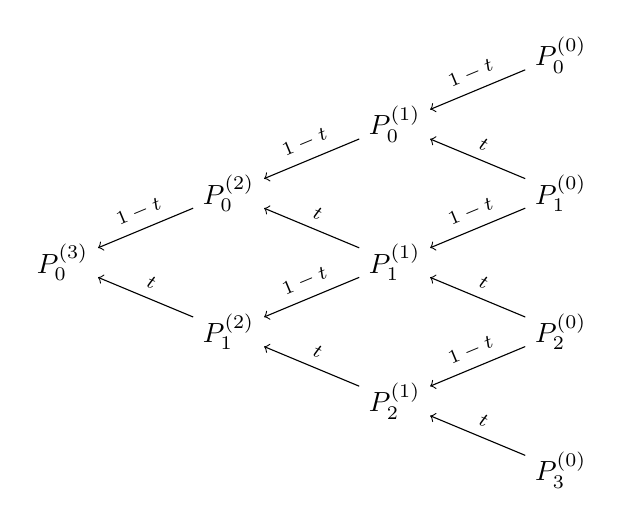
\begin{tikzpicture}
		\def\dx{60pt}
		\def\dy{25pt}

		\pgfmathsetmacro{\numcontrolpoints}{3}

		\newcounter{i}
		\newcounter{j}
		

		\node (\arabic{i}) at (0,0) {$P^{(\numcontrolpoints)}_0$};
		\stepcounter{i}

		\foreach \x in {1, ..., \numcontrolpoints} {
			\pgfmathsetmacro{\xstep}{\x-2}

			\setcounter{j}{0}
			\foreach \y in {\x, \xstep, ..., -\x} {
				\pgfmathsetmacro{\psuperscript}{\numcontrolpoints-\x}
				
				\node (\arabic{i}) at (\x*\dx, \y*\dy) {$P^{(\pgfmathint{\psuperscript}\pgfmathresult)}_{\arabic{j}}$};
				\stepcounter{i}
				\stepcounter{j}
			}
		}


		\newcounter{z}
		\newcounter{a}
		\newcounter{b}
		\pgfmathsetmacro{\maxx}{\numcontrolpoints}
		\foreach \x in {1,...,\numcontrolpoints}{
			\foreach \y in {1,...,\x}{
				
				\setcounter{a}{\arabic{z}}
				\addtocounter{a}{\x}

				\setcounter{b}{\arabic{z}}
				\addtocounter{b}{\x}
				\stepcounter{b}
				
				\draw [<-] (\arabic{z}) -- (\arabic{a}) node[above, midway, sloped] {\scriptsize $1-t$};
				\draw [<-] (\arabic{z}) -- (\arabic{b}) node[above, midway, sloped] {\scriptsize $t$};
				
				\stepcounter{z}
			}
		}
	\end{tikzpicture}
	\caption{Beziér curves of different degrees and their control points}
\end{figure}

\begin{figure}[!ht]
	\centering
	\includesvg[width=\textwidth]{../python/deCasteljauVisual}
	\caption{Beziér curves of different degrees and their control points}
\end{figure}



\subsection{Properties}

\begin{figure}[!ht]
	\centering
	\includesvg[width=\textwidth]{../python/bezierDifferentDegrees}
	\caption{Beziér curves of different degrees and their control points}
\end{figure}



\section{Non-Uniform Rational B-Splines (NURBS)}
\subsection{Definition}
\subsection{Properties}
\subsection{De Boor's Algorithm}

\section{Methods on NURBS Objects}
\subsection{Affine Transformations}
\subsection{The Frenet-Serret Apparatus}
\subsection{Finding Intersections}
\subsection{Interpolation}

\section{Jet Engine Design Specifics}
\subsection{Fundamental Terms}
\subsection{The S2M Net}
\subsection{Fillet Creation}

\chapter{Results}
\section{Cooling Geometries And Their Parametrizations}
\subsection{Chambers}
\subsection{Turnarounds}
\subsection{Slots}
\subsection{Film Cooling Holes}
\begin{figure}[!ht]
	\centering
	\includesvg[width=0.5\textwidth]{../python/fanshapedCurveDefinition}
	\caption{yeah}
\end{figure}
\begin{figure}[!ht]
	\centering
	\includesvg[width=0.5\textwidth]{../assets/tecplot/selfIntersection}
	\caption{yeah}
\end{figure}


\subsection{Impingement Inserts}
\section{Export for CENTAUR}
\section{Export for Open CASCADE}

\chapter{Discussion}
\section{Future Work}
\section{Conclusion}
\cite{Piegl1997}

% Bibliography, numbered and formatted like a chapter (for the TOC as well)
\printbibliography[heading=bibnumbered, title=References]

\end{document}